% Chapter4
\chapter{Implementierung} \label{chapter:thevetestcase}
\section{Modellierung der Anlage}
Für das Aufbauen einer Anlage, ist ein vorab überlegtes Konzept von großer Bedeutung. Mittels des Rohr- und Instrumentenfließschemas wird ein später noch des öfteren abgeändertes Abbild erstellt. Die in der Anfangsphase aufkommenden Änderungen ergeben sich angesichts der nur partiellen Implementierung der Anforderungen. Initial wird hoher Wert auf Redundanzen gelegt. Erst eine größere Anzahl an Bauteilen kann einen parallelen Ablauf mehrerer Arbeitsschritte ermöglichen. Durch die drei eingebauten Tanks und zwei Reaktoren, die mittels der drei Hauptleitungen verbunden sind, ist das Umfüllen zwischen zwei Tanks, sowie das gleichzeitige Befördern von Flüssigkeit vom dritten Tank in einen der Reaktoren möglich.\\

Die zwei Pumpen sind so platziert, dass bei einem eventuell auftretenden Defekt die andere Pumpe deren Aufgabe übernehmen kann. Arbeitsschritte können dadurch zwar nur noch sequentiell abgearbeitet werden, jedoch kommt es nicht gleich zu einem totalen Ausfall der Funktionalität der Anlage. Eine weitere Absicherung gegen möglich aufkommende Störfälle ist die Position der Tanks. Durch ihre Lokalisation an der höchsten Stelle der Apparatur besteht die Opportunität die Schwerkraft zu nutzen.\\

\begin{figure}[h!]
  \centering
  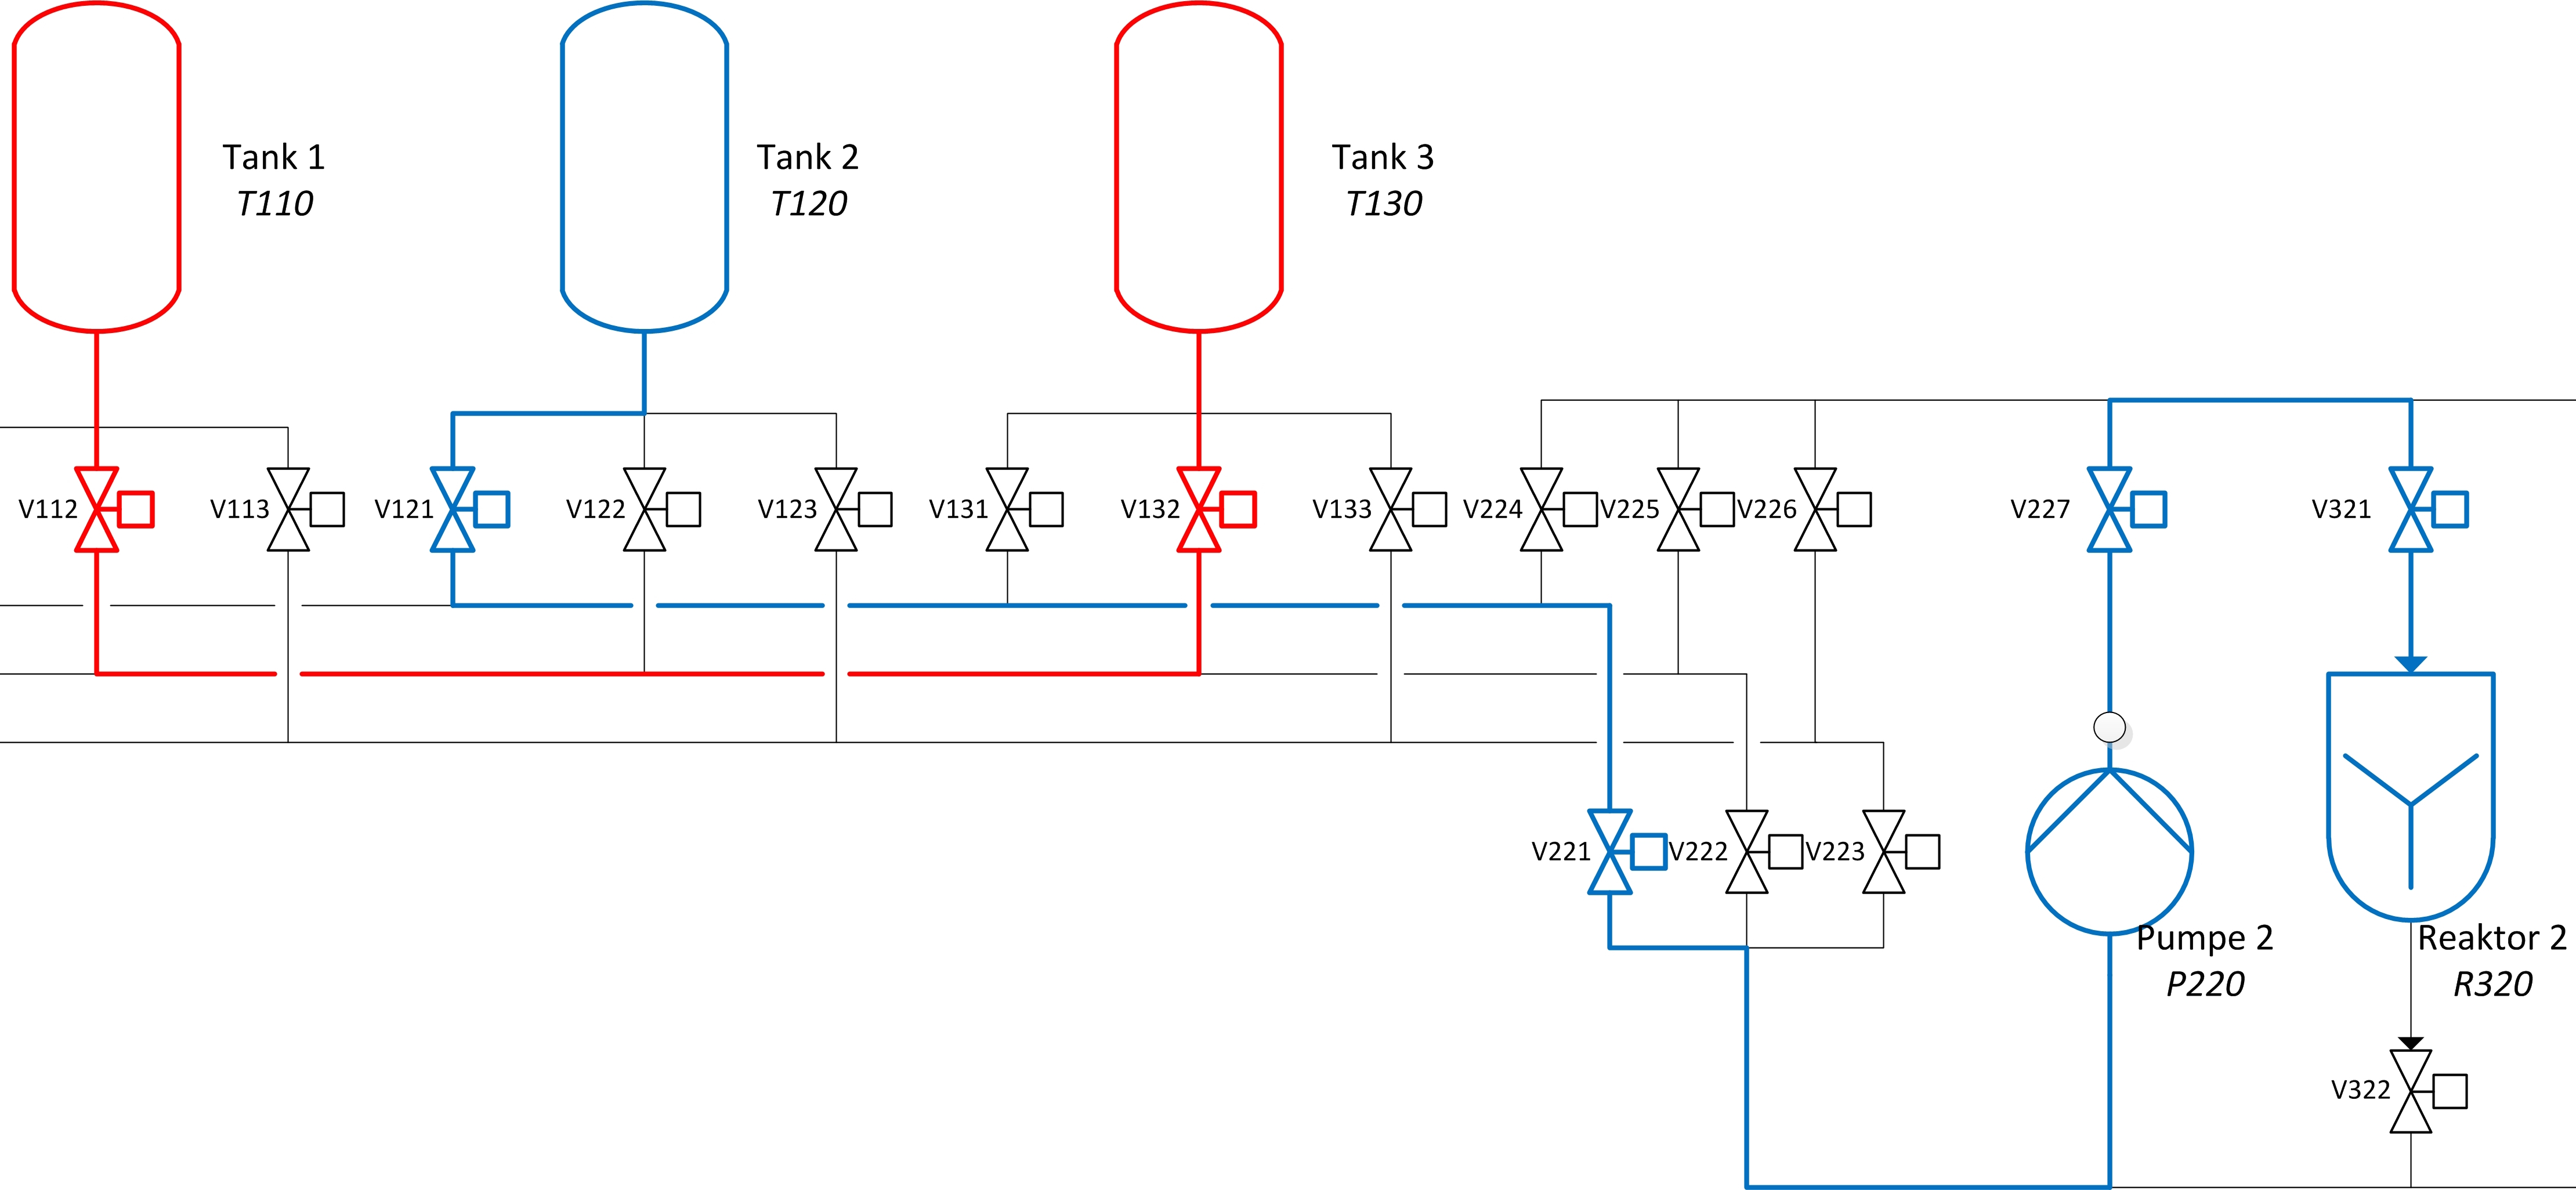
\includegraphics[width=1\textwidth]{graphics/implementation/RI_Impl_cropped.jpg}
  \caption{Mögliche Parallelität im RI ersichtlich}
\end{figure}

Jedes Ventil hat eine vorteilhafte Durchflussrichtung, die meistens mit einem Pfeil direkt auf dem Bauteil gekennzeichnet ist. Ganz abgesehen davon, ob es sich um ein Ventil handelt, welches im stromlosen Zustand geschlossen ist oder ob es ein schließendes Ventil ist, diese Vorgabe sollte stets eingehalten werden. Aspekte wie dieser haben in die Modellierung der Anlage selbstverständlich eingebaut zu werden.\\

\todo[inline]{BILD EINFÜGEN}

\begin{figure}[h!]
  \centering
  %\includegraphics[width=0.7\textwidth]{graphics/implementation/BILD}
  \caption{Ventil mit vorteilhafter Fließrichtung}
\end{figure}

Um in der Anlage befindliche Flüssigkeiten zu entfernen, muss ein eigens für den Auslass vorgesehenes Ventil installiert werden. Vorteilhafterweise handelt es sich bei der Position dieses Bauteils um den tiefsten Punkt der Apperetur. Alternativ dazu kann dieses auch direkt nach einer Pumpe montiert werden.

\section{Aufbau der Anlage}
Auf Basis des Rohr- und Instrumentenfließschemas kristallisiert sich eine exakte Anzahl an benötigten Bauteilen heraus. Für den noch bevorstehenden Aufbau der Anlage ist zu beachten, dass beim Auswählen der Einzelteile alles kompatibel sein muss. Nicht vorhandene Vereinbarkeit kann vor allem für diesen speziellen Anwendungszweck zu katastrophalen Auswirkungen führen, da einerseits mit Flüssigkeiten gearbeitet wird, sowie gleichzeitig stromdurchflossene Leitungen existieren. Eine Verbindung dieser genannten Komponenten hätte irreparable Schäden zur Folge. Im Rahmen einer übergeordneten Forschungsarbeit wurde diesem Projekt ein Budget von 6000 \todo{Euro} \euro \space zugesprochen. Die Auswahl der benötigten Teile hat verständlicherweise im Rahmen dieser beschränkten Geldmittel zu geschehen.\\
	
	Für einige verwendete Element gibt es spezifische Parameter, die auf jeden Fall einzuhalten sind:\\
	
	\textbf{Ventile:}\\
	Ein ausschlaggebendes Kriterium der verwendeten Ventile ist, dass sie in stromlosem Zustand geschlossen sind. Im Falle eines Ausfalls der Energieversorgung kann somit sichergestellt werden, dass sich alle Verbindungen aus Schutz vor Flüssigkeitsverlust schließen. Für die Funktion der Nutzung der Schwerkraft zum Umleiten von Flüssigkeiten ist auch relevant Ventile zu haben, die keinerlei Vordruck benötigen um den Durchfluss zu gewähren.\\

	\textbf{Tanks:}\\
	Abgesehen von einem für Testzwecke vernünftigen Füllvolumen ist es erforderlich einen Tank zu wählen, dessen Ausgang sich am niedrigsten Punkt befindet. Andernfalls kann man nur bedingt Nutzen aus der Schwerkraftsteuerung ziehen.\\
	
	\textbf{Pumpen:}\\
	Mit Hilfe eines Gleichstrom - Wandlers muss es möglich sein, die Pumpen mit dem zur Verfügung stehenden Ausgangstrom der SPS von 0 bis 10 Volt zu betreiben.\\
	
	\textbf{Rohre:}\\
	Die Rohre müssen jedenfalls dem Druck der Pumpen standhalten können. Desweiteren ist das exakt abzustimmende Einpassen in die Ventile, um Dichte gewährleisten zu können, ein wichtiger Parameter.\\

	Die bereits bei der Bestellung bekannten, tatsächlichen Maße der Bauteile, haben einen relevanten Einfluss auf den finalen Aufbau. Da es auch bei der Profilplatte physikalische Grenzen gibt, muss die endgültige Positionierung genauestens überlegt ausfallen. Der zukünftigen Vereinfachung des Aufbaus der Produktionsanlage halber, wurde daher projektintern beschlossen, ein kleines Modell der Apparatur zu erstellen. Da aus dem Rohr- \& Instrumentenfließschema keinerlei Information zur endgültigen Lokalisation der Bauteile ersichtlich ist, wird ein erster physikalischer Entwurf konstruiert. Mit Hilfe diesem können Abstände zueinander stehender Elemente deutlich gemacht werden. Realisiert wird der genannte Prototyp mit leicht zugänglichen Arbeitsmaterialien wie etwa Trinkhalme, Papier und Klebeband.\\
	
		\todo {Bild des Miniaturmodells}

	Für den tatsächlichen Aufbau ergibt sich günstigerweise die Möglichkeit, mechanische Anforderungen mit Hilfe der technischen Werkstätte abzuwickeln. Profilschienen, die als stabilisierendes Gerüst dienen, werden penibelst mit der Aluminiumsäge auf das gewünschte Maß geschnitten. Im späteren Verlauf werden diese samt den Tanks zum ersten aufgebauten Teil der Anlage. Für die Verbindung der Tanks, Pumpen, Ventile und Reaktoren dienen undurchsichtige Kunststoffrohre. Um gewährleisten zu können, dass die Verbindung absolute dicht ist, müssen die Rohre unbedingt gerade geschnitten sein. Abermals dürfen dafür Maschinen der mechanischen Werkstatt verwendet werden. Erst mit einer Bandsäge grob vorgeschnittene Rohrstücke werden in eine konventionelle Drehmaschine eingespannt. Mit einem scharf angeschliffenen Drehstahl ist es möglich, den unsauberen Schnitt absolut plan zu gestalten. Nachdem abschließend einzelne Komponenten noch entgratet werden, ist die Arbeit an den Rohren zur Verbindung getan.\\
	
	Verbundungen mit den ersten neun Ventilen der Hauptleitungen und den Tanks können ab sofort verlegt werden.\\
	
		\todo[inline]{Bild: Erster Aufbau (Tanks, Hauptpipes)}
		
	Das Einbauen der bestellten Pumpen gestaltet sich komplizierter als gedacht, da die ursprüngliche Bestellung einen Fehler beinhaltet. Nur eines der beiden gelieferten Modelle entspricht der gestellten Anforderung, was einschließlich der Rücksendung weitere wertvolle Zeit kostet. Unterdessen kann die zweite Pumpe verbaut werden. Funktionale Bauteile dieser Art sind bei der zeitgemäßen verfügbaren Leistung gut gedämpft. Angesichts der Tatsache, dass man mit dieser bis zu 30 Meter hoch pumpen könnte, befindet sich auf der Unterseite ein gummiertes Verbindungsstück, um bei Inbetriebnahme die stärksten Vibrationen abfangen zu können. Mit vom Profilschienen Schneiden übergebliebenen Reststücken wird eine Konstruktion gebaut, um die Höhe der Pumpe mit der der Rohre gleichzusetzen. Unmittelbar nach der Pumpe wird ein Durchflusssensor angebracht, der im späteren Verlauf des Projekts zur automatischen Steuerung beitragen soll.
	
	Abermals in der Werkstatt genauest zugeschnittene Profilschienen ergeben eine Konstruktion zur Aufhängung der Reaktoren. Das beste Beispiel der Bauteil-Positionsuntreue eines Rohr- \& Instrumentenfließschemas ist anhand des aufkommenden Arbeitsschritts zu sehen. Ursprünglich sind die beiden Reaktoren seitlich der restlichen Anlage platziert. Da es die Profilplatte aber nicht zulässt, da sie nur eine gewisse Breite hat, müssen diese in den Vordergrund geholt werden. Bei der Bauart der Reaktoraufhängung ist zu beachten, dass das größt möglich aufkommende Gewicht ausschließlich dort zustande kommen kann, da Reaktoren zum Mischen mehrerer Tankinhalte verwendet werden können. Diese Überlegung muss jedenfalls dazu beitragen, ausreichend Stabilität und Belastungsfähigkeit zu erlangen.\\
	
	Die bereits eingebauten Ventile besitzen jeweils zwei Phasen und eine Masse. Die Verkabelung selbst wird mit einem starren 3-Phasen-Kabel umgesetzt, da über eine flexibles Litzenverbindung nicht so viel Strom geleitet \todo{Stimmt das?}  werden sollte. Aus Gründen der Übersichtlichkeit wird jedes Kabel sowie Ventil beschriftet, um eventuell aufkommende Komplikationen zu unterbinden. In den Rillen der Profilschienen verlegt, werden alle mit Kabelbindern verbundene Leiter zur SPS zurückgeführt. Im späteren Verlauf eines Folgeprojekts soll eine Verlegung der SPS an die Unterseite des Tisches geschehen, weshalb es ausschlaggebend ist, alle Kabel mit einem deutlichen Übermaß zu schneiden. Die deutlich beschrifteten Kabel können anschließend der Funktionalität des jeweiligen Bauteils entsprechend in den dafür konzipierten SPS-Slot eingebaut werden.\\
	
	Mit dem Einbau der Füllstandssensoren in den drei Tanks sind die letzten Arbeitsschritte des physikalischen Aufbaus der Anlage getan.

\section{Phasen und Rezepte}
	Der Begriff Prozedur beschreibt das Zusammenfassen mehrerer Grundfunktionen einer Anlage, um einen Ablauf zu automatisieren. Das Gegenspiel zwischen der Software zenon und der SPS kann als sogenannte \glqq State-Machine \grqq \space betrachtet werden. Da eine SPS dem zyklischen Abarbeiten programmierter Funktionen unterliegt, ist es ein ständiges Nachfragen ob ein jeweiliger Zustand schon erreicht wurde. Durch global gesetzte Status kann so ein automatischer Wechsel der ausgeführten Funktionen erfolgen. Als Rezept wird das Aneinanderreihen mehrerer Prozeduren bezeichnet, um einen weiteren Schritt der Automatisierung zu gehen.\\

\begin{figure}[h!]
  \centering
  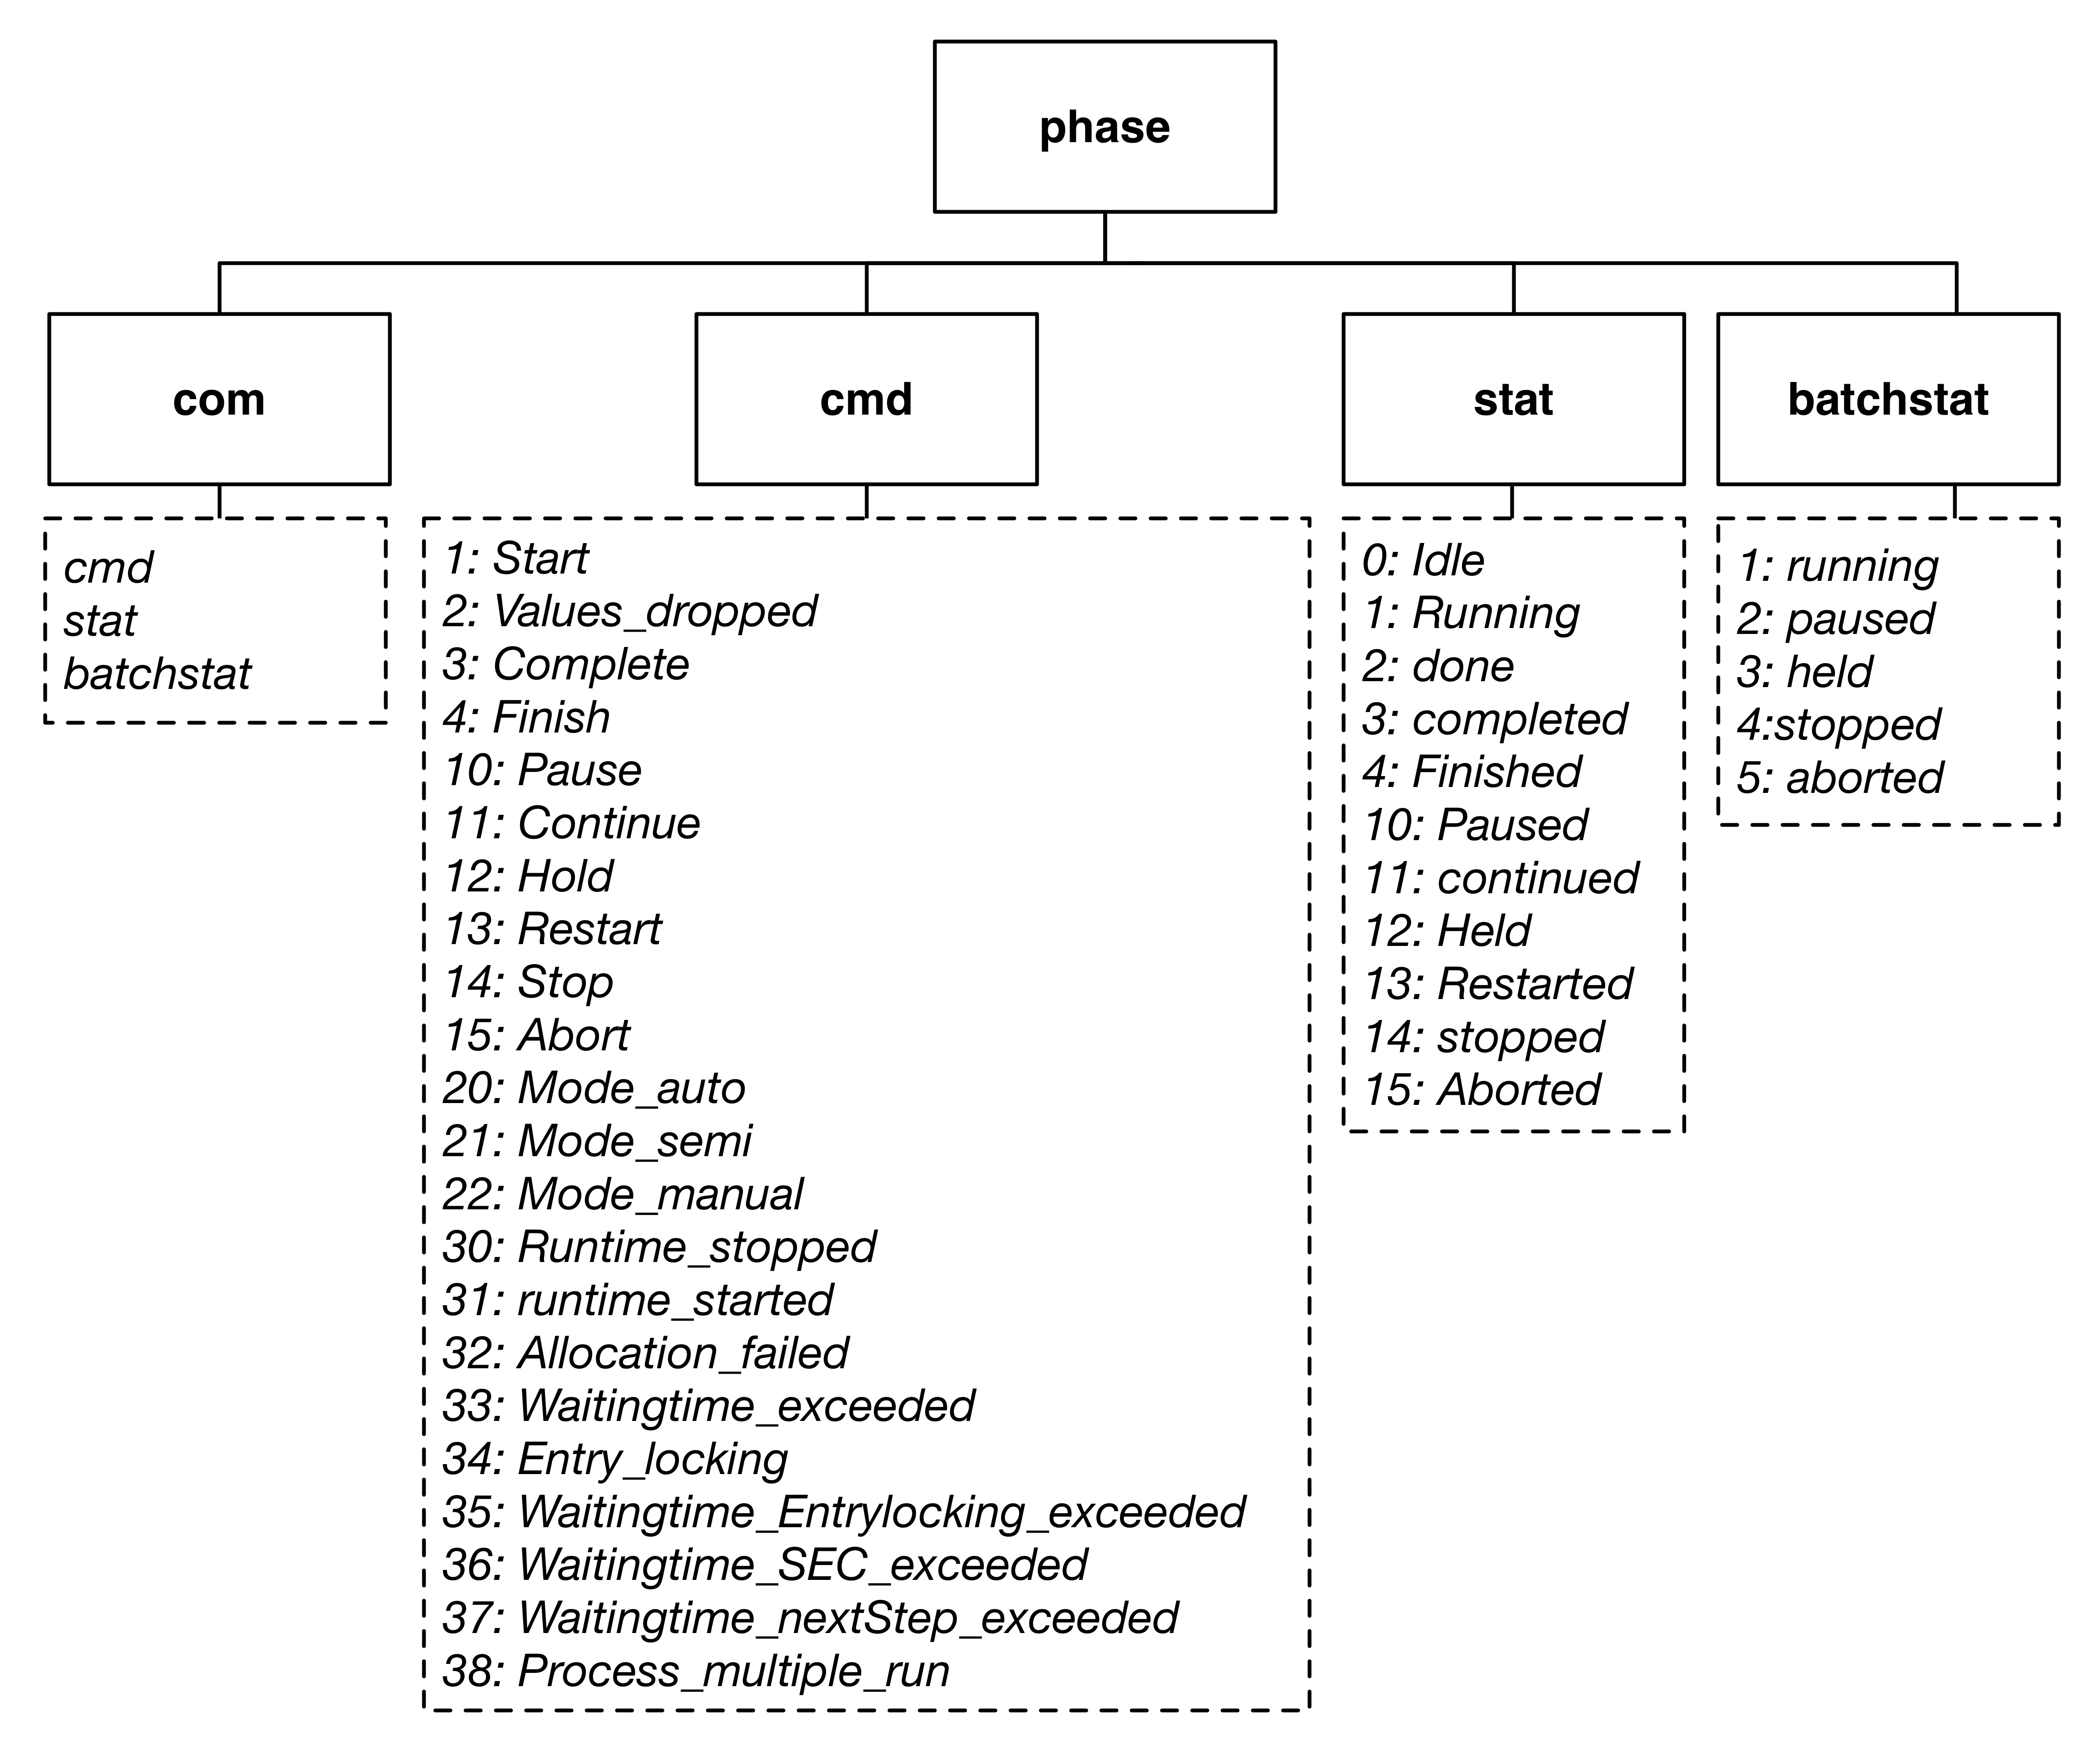
\includegraphics[height=0.6\textwidth]{graphics/implementation/Datentyp_Phase.jpg}
  \caption{Aufbau der Strukturvariable \glqq \textit{phase}\grqq}
\end{figure}
	
	Für die Kommunikation zwischen einer Prozedur bzw. eines Rezepts und der SPS stehen drei Variablen zur Verfügung
	
	\begin{itemize}
		\item Kommando: Sendet Befehle an SPS-Grundfunktion
		\item Status: Empfängt internen Status der SPS-Grundfunktion
		\item Batchstatus: Sendet internen Status des Rezepts zur SPS
	\end{itemize}

	Kommando trägt der SPS auf, was getan werden muss. Mit dem Status wird der Software zenon mitgeteilt, in welchem Stadium sich die Prozedur gerade befindet. Die Variable Batchstatus teilt mit, wo im gesamt abzulaufenden Programmcode sich die SPS gerade befindet.\\
	
	Um eine Prozedur in zenon zu konfigurieren, benötigt es eine ganze Anzahl an zu erledigenden Arbeitsschritten, die da wären:\\

	Initialisierend wird im Unterpunkt Batch Control ein neues Aggregat mit einer sich darin befindlichen neuen Grundfunktion (Prozedur) angelegt. Die Prozedur benötigt nun die zuvor erwähnten Kommunikationsvariablen Status, Command und BatchCommand. Zu beachten ist allerdings, dass es diese Strukturvariable bereits in der Form \glqq \textbf{name}.com.* \grqq \space gibt. Abermals untergeordnete Reaktionen werden mit den gewünschten Ereignissen befüllt, wobei wiederum zu beachten ist, dass diese den richtigen Variablen zugeordnet sein müssen.\\

	Weitere Arbeitsschritte werden mit mittels Zenon Logic abgearbeitet. Ein Hauptprogramm, welches zum Ausführen aller anderen Funktionen dient, wird angelegt. Aufgerufene Unterprogramme sind get\_cmd(), get\_batchstat(), die auszuführende(n) Prozedure(n) und send\_state() und müssen vor dem ersten Durchlauf des Hauptprogramms angelegt sein.\\
	
	\textbf{get\_cmd()}\\
	Null setzen (\glqq false\grqq \space setzen) aller Boolean-Werte, die einen Status repräsentieren, um alles zurückzusetzen, sowie durchgehen aller zur Auswahl stehenden Kommandos und setzen der Variable des zutreffenden Kommandos (\glqq true\grqq \space setzen).\\

	\textbf{get\_batchstat()}\\
		Zutreffender aktueller Status der Grundfunktion wird gesetzt.\\

	\textbf{Prozedur}\\
		Variablen bis zur Abbruchbedingung setzen\\

	\textbf{send\_state()}\\
		Globales Setzen des aktuellen Status
		
\begin{figure}[h!]
  \centering
  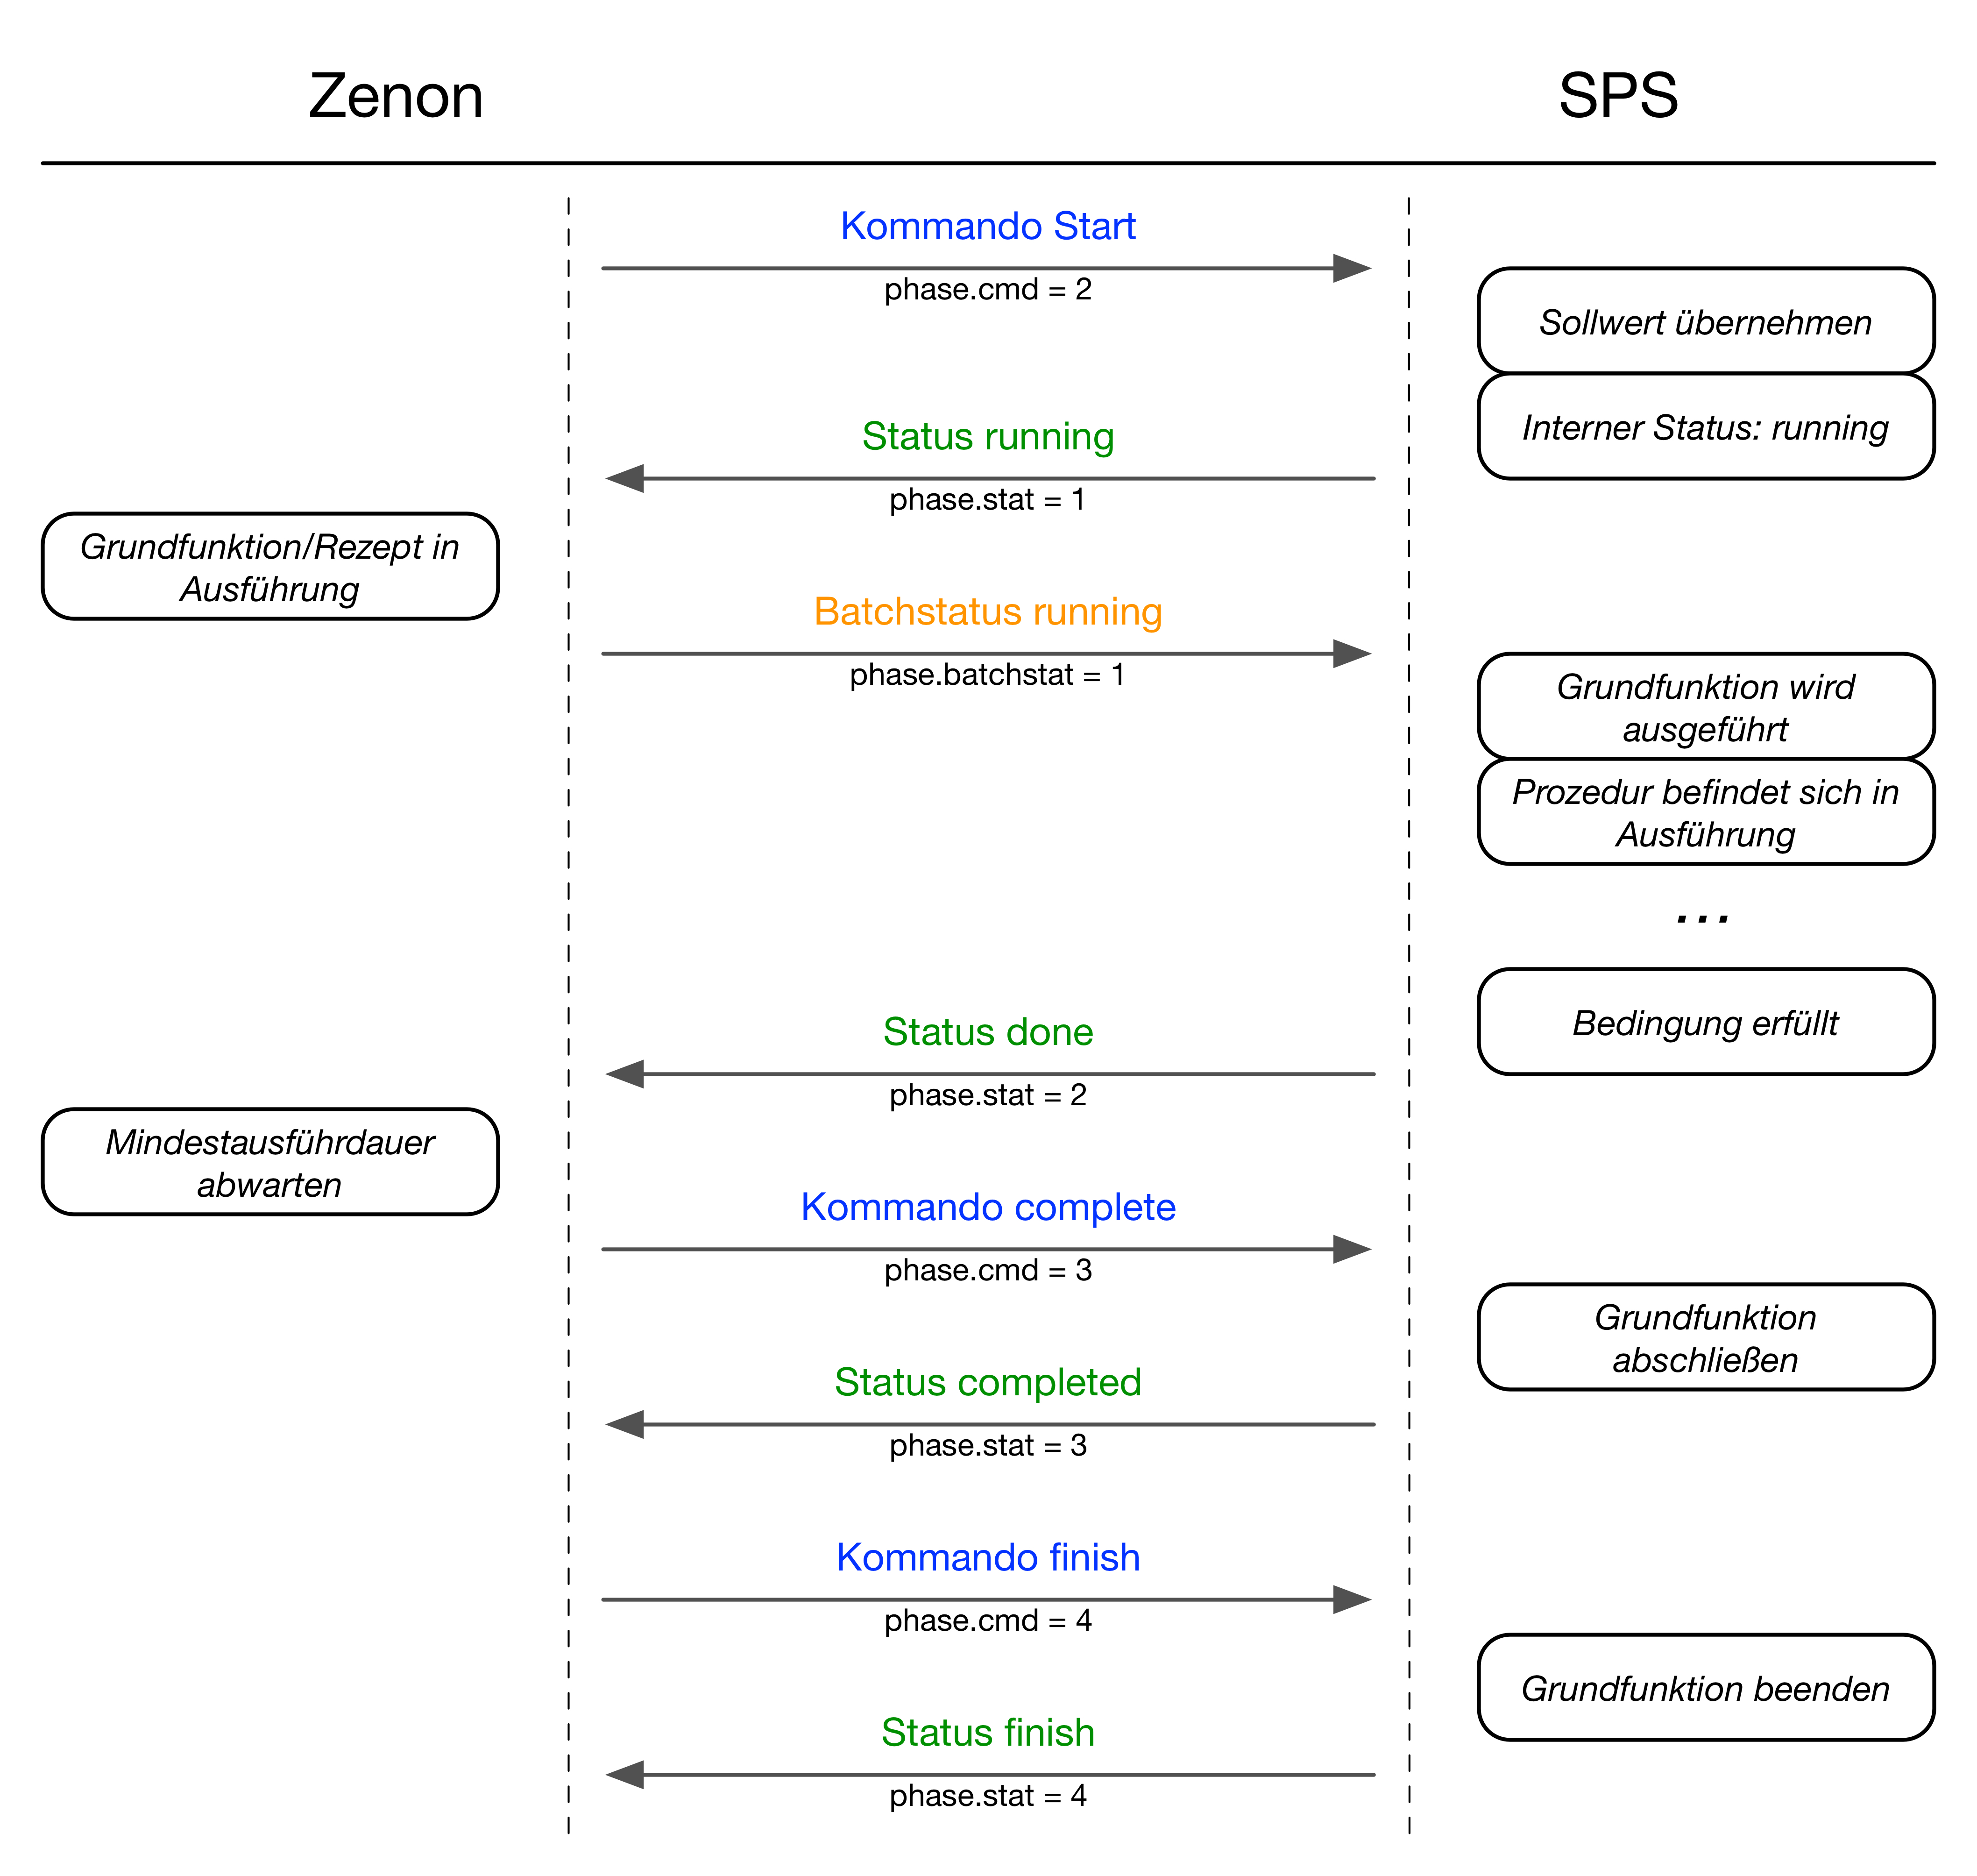
\includegraphics[height=0.95\textwidth]{graphics/implementation/StateMachine.jpg}
  \caption{Kommunikationsmodell von zenon und SPS}
\end{figure}

\section{HMI}
Für dieses Projekt wurde als SCADA System die Software zenon vorgegeben, daher wird das HMI in zenon Supervisor (zenons HMI Programm) umgesetzt.\\
\\
\textbf{Visualisierung}\\
In zenon wird eine Visualisierung \glqq Bild\grqq\space  gennant. Dieses kann mit vorgefertigten Elementen erweitert werden. 

Als Ausgangspunkt für die Visualisierung wurde das RI-Fließeschema zur Hand genommen. Aus diesem wurde die Anzahl der Elemente und die Grundstruktur übernommen. Als nächsten Schritt musste evaluiert werden, welche Inhalte des RI-Fließschemas für die Visualisierung relevant und welche Informationen nicht vorhanden waren.\\
\\
\textbf{Feldbuskonfiguration}\\
Um eine Visualisierung mit aktuellen Sensorwerten zu befüllen, wird eine Verbindung zur SPS benötigt. Diese Verbindung wird über das Teilprogramm zenon Logic (im weiteren nur noch Logic genannt) hergestellt.\\
\\
Als ersten Schritt, um in Logic eine SPS hinzuzufügen, muss im Unterpunkt \glqq Feldbuskonfiguration\grqq\space die Treibersoftware für die ADAM5550 SPS hinzugefügt werden. Daraufhin müssen alle Module, die an der SPS angebracht sind, in die Konfiguration hinzugefügt werden.\\%todo Position
\begin{figure}[h!]
  \centering
  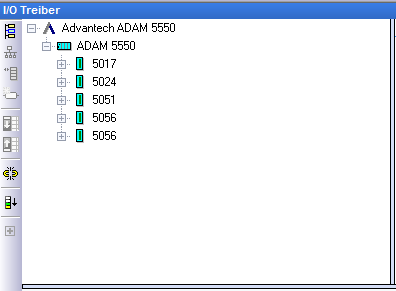
\includegraphics[width=0.7\textwidth]{graphics/implementation/Feldbuskonfiguration}
  \caption{Feldbuskonfiguration}%todo Grafik name
\end{figure}
\\
\textbf{Variablen}\\
In zenon können auf mehrere Arten Variablen erstellt werden. Damit diese für die Visualisierung und von Logic sichtbar sind, müssen sie als Globale Variable definiert werden. Der einfachste Weg dafür ist es, im Logic Variablenfenster, über den Reiter  \glqq Globale Variablen\grqq, die Funktion \glqq Variable hinzufügen\grqq\space aufzurufen.\\%todo Position
\begin{figure}[h!]
  \centering
  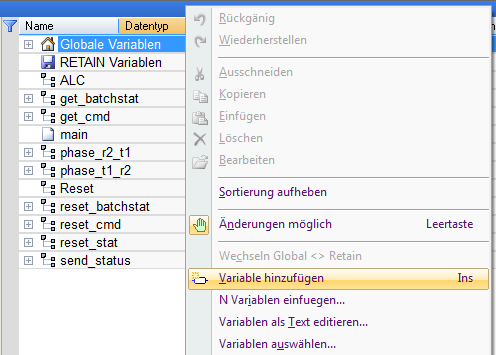
\includegraphics[width=0.7\textwidth]{graphics/implementation/Variablen}
  \caption{Variablen}%todo Grafik name
\end{figure}\\
Sobald alle Variablen erstellt sind, werden diese mit der Feldbuskonfiguration verknüpft. Durch diesen Schritt erhält man Zugang zu den an der SPS angeschlossenen Bauteilen.\\
%Die erstellten Variablen mussten als nächstes in der Visualisierung eingetragen werden um in dieser im nächsten Schritt eine Steuerung zu erzeugen.\\
\\
%Feldbuskonfiguration -> Konfiguration einfügen (Advantech ADAM 5550) -> Master/Port hinzufügen (ADAM 5550) -> Slave/Datenblock einfügen (Slot:Steckplatz an SPS; Module: Analog/Digital|In/Out|4/8/16 Channels...) -> Variable hinzufügen (Channel; Variablenname)
%Variable -> Globale Variable hinzufügen (erzeugt Variable in logic und auch im supervisor zugänglich für die Visualisierung) -> In Visualisierung zu den Elemente die richtigen Variablen hinzufügen -> Bei Feldbbuskonfiguration bei richtiger I/O auf richtigem Channel hinzufügen
%TEST -> logic Programm hochladen -> Variablen in logic zeigen aktuelle werte an -> check mit werten direkt von der SPS

%Umrechnen von Sensorwerten: 
%Durchflusssensor Digital -> etwa 900 ticks pro Liter -> Timer bid 900 ticks -> Liter/min
%Füllstandsensor 4-20mA -> 4=voll, 20=leer -> Variablen/Tank Konfiguration -> Umrechnung 4=100, 20=0
%Ventilstatus 0/1 -> Variablen Konfiguration -> Extremwerte farblich markieren -> Ventil Elementfarbe nach Variablen Farbe
\textbf{Steuerung}\\
\\
Phase 1 Steuerung mittels Buttons\\
	Der erste Versuch war es die Steuerung mittels einfachen Buttons umzusetzen. Diese haben meist die in zenon vorhandene Funktion  \glqq Sollwert absetzen\grqq\space  verwendet, welche den Wert einer Variable ändert.\\
	So konnten alle Funktionen umgesetzt werden, dadurch erhielt das  \glqq Bild\grqq\space  jedoch viele Elemente die von der Eigentlichen Visualisierung ablenkten.\\
\\
Phase 2 Versteckte Buttons\\
	Um den Element-Overload zu verringern war der nächste Schritt die Button zu  \glqq verstecken\grqq\space  indem sie Transparent über die eigentlichen Elementen (beispielsweise ein Ventil) verschoben wurden.\\
	In der Visualisierung wurden nun weniger  \glqq unwichtige\grqq\space  Bausteine angezeigt, die Elemente waren jedoch immer noch da, wodurch die Größe (MB) der Visualisierung deutlich anstieg.\\
\\
Phase 3 Funktionale Elemente\\
	Der nächste schritt war es die nicht funktionalen Grafikelemente durch Buttons in Form der gewünschten Elemente zu ersetzten.\\
\\
\textbf{Rezepterstellung}\\
%todo Rezeperstellung

\section{Ontology}
Nachdem die Evaluierung der wichtigsten Aspekte im Kapitel Ontologie der Chargenprozessanlage in Hinsicht auf eine automatisierte Codegenerierung durchgeführt wurden, behandelt dieses Kapitel den Werdegang der Ontologie vom Ersten bis hin zum Finalem Design.\\
\\
Das Ziel der Ontologie ist es, die im laufe dieses Projekts aufgebaute Anlage in einer Art und Weise abbilden zu können, die es erlaubt daraus eine automatisierte Codegenerierung durchzuführen und dabei auf einem Abstraktionslevel zu bleiben um einen Großteil an in der Industrie vorkommenden Produktionsanlagen abbilden zu können.\\
\\
Da es den Rahmen dieser Arbeit sprengen würde, auf jeden einzelnen Gedankengang in der Erstellung der Ontologie einzugehen, werden nur die großen Revisionen der Ontologie genauer beschrieben.\\
\\
Zu aller erste werden alle Bauteile der Anlage in Kategorien eingeteilt.\\
Tanks, Reaktoren und Pumpen sind die Hauptelemente dieser Anlage und werden deswegen auch in einer Gruppe zusammengefasst. Neben ihnen gibt es eine Gruppe an Bauteilen die etwas tun, hierzu gehören die Ventile, Sensoren, Heiz- und Rührstäbe. Die restlichen Elemente der Anlage sind Statische Objekte die einen Nutzen besitzen, jedoch keine Arbeit erledigen, daher fallen diese zusammen unter die Kategorie von Passiven Elementen. Zu diesem Zeitpunkt sind dies nur die Rohre.\\
Eine Ausnahme dieser Gruppen ist die SPS welche etwas tut, daher an sich in Kategorie 2 Fallen würde, aber nicht direkt Teil der Anlage ist und daher auch als einzelstehendes Objekt einen Platz in der Ontologie findet.

\begin{figure}[hbt!]
  \centering
  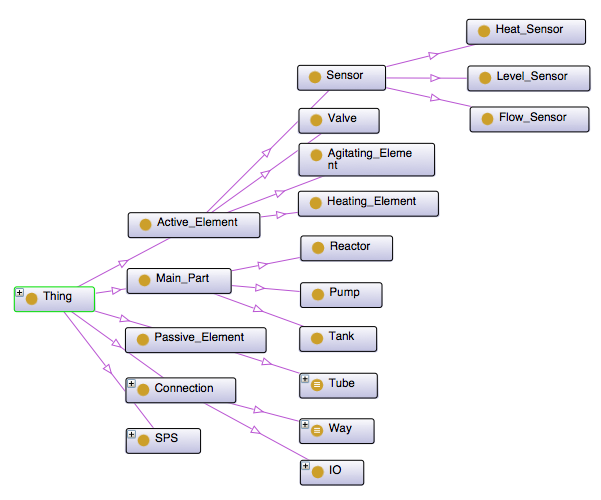
\includegraphics[width=0.6\textwidth]{graphics/implementation/Ontology_v1}
  \caption{Erste Version der Ontologie}
\end{figure}

Verbindungen zwischen 2 Klassen werden normalerweise mit einer Objekt Eigenschaft dargestellt, da eine Verbindung zwischen 2 Bauteilen aber eine andere Information als die Verbindung zwischen einer SPS und einem Bauteil enthält, gibt es die Kategorie Connections mit den Klassen “Weg” und “IO”.

Kurz zusammengefasst können die Kategorien wie folgt beschreiben werden\\
Main\_Part:\\
	Dies sind alle Elemente die subjektiv als Hauptelemente bezeichnet werden.\\
Active\_Element:\\
	Jene Bauteile die etwas tun - Aktuatoren, Sensoren\\
Passive\_Elements:\\
	In der Anlage verbaute teile die keine Arbeit verrichten.\\ 
Connection:\\
	Verbindungsarten zwischen den einzelnen Bauteilen\\
\\
Mit dieser Ontologie ist es grundsätzlich möglich die Anlage aus Kapitel 4.2 abzubilden, jedoch finden sich einige Inkonsistenzen die die automatisierte Codegenerierung erschweren wenn nicht sogar unmöglich machen würden.\\
\\
%Die nächste Version befasst sich damit die einzelnen Kategorien genauer zu bestimmen, um einen Konsistenten zustand in die Ontologie zu bringen, gleichzeitig aber auch eine Struktur zu bilden die eine automatische Codegenerierung erleichtert.
Nun wird die erste Version der Ontologie, in Hinsicht einer automatisierten Codegenerierung, evaluiert und dementsprechend umgebaut.\\
Die Kategorien werden im nächsten Schritt genauer definiert um eine Konsistenz in die Ontologie zu bringen.\\
\\
Die definition von \glqq Active\_Element\grqq\space ist in Grunde richtig, nur beinhaltet diese die SPS was nicht der Fall sein soll. Daher wird die Definition auf \glqq Elemente die mit einer SPS (I/O) verbunden sind\grqq\space geändert. In diese Kategorie fallen nun die Elemente der Ersten Version ohne SPS und auch die Pumpe hinein.\\
\\
Die nächste Kategorie die bearbeitet wird ist \glqq Main Part\grqq\space. Die Definition in dieser Gruppe ist noch sehr grob definiert und lässt eine Subjektive Gruppierung zu, daher muss die Definition von Grund auf geändert werden ohne Bauteile die zurzeit Enthalten sind auszuschließen. Die passende Interpretation ist \glqq Elemente mit mindestens 2 Ein bzw. Ausgängen\grqq\space. Durch diese Änderung fallen nun auch die Ventile in die Gruppe \glqq Main Part\grqq\space.\\
\\
Um Ein-/Ausgänge besser zu definieren wird die Gruppe \glqq Connection\grqq\space verändert. Die Klasse \glqq I/O\grqq\space wird heraus genommen da man diese genauer beschreiben muss. Dadurch enthält \glqq Connection\grqq\space nur noch Verbindungen zwischen Bauteilen, welche nur noch Ein-/Ausgänge sein können.\\
\\
Die Kategorie \glqq Passive Element\grqq\space wird komplett entfernt da sie keine Relevanten Information enthält.

\begin{figure}[hbt!]
  \centering
  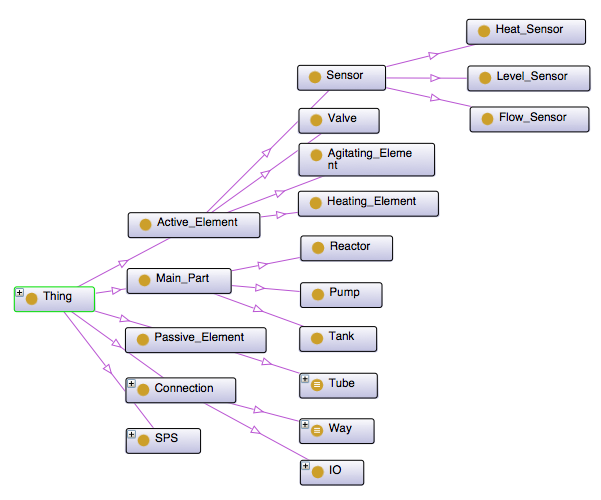
\includegraphics[width=0.6\textwidth]{graphics/implementation/Ontology_v2}
  \caption{Erste Überarbeitung der Ontologie}
\end{figure}

\textbf{Object Properties}\\
\\
Nachdem die Klassenstruktur feststeht, müssen als nächstes die Relationen bestimmt werden.
\begin{table}[h]
\centering
\begin{tabular}{l|l|l}
\textbf{Name} & \textbf{Domain} & \textbf{Range} \\ \hline
hasActiveE    & Input, Output   & Active\_Element \\ \hline
hasConnection & MainPart        & Connection      \\ \hline
hasIO         & Thing           & Input, Output   \\ \hline
includes      & Tank            & Active\_Element \\ \hline
isConnectedTo & Connection      & Connection                            
\end{tabular}
\end{table}
\\
\textbf{Data Properties}\\
TODO
\section{Aktivitätsdiagramm}
TODO
\section{Codegenerierung}

TODO